%-------------------------------------------------------------------------------
%	PREFAZIONE 
%-------------------------------------------------------------------------------
\thispagestyle{empty}
\chapter*{Prefazione}
L'alone di mistero che avvolgeva la morte di Mingazzi mi appassionò a tal punto da spingermi a cercare di scoprire sempre più dettagli sulla storia della mia famiglia e del mio paese. Cominciai a costruire l'albero genealogico di tutta la famiglia cercando di raccogliere anche testimonianze e dettagli su certi parenti. La figura di Stefano Mingazzi mi ha incuriosito particolarmente e ho voluto approfondire intervistando mia nonna chiedendole tutto ciò che ricordava. Dopo la morte di mio nonno Elio, io e mio fratello Riccardo cominciammo a perlustrare ogni singolo centimetro del suo studio. Qualche giorno dopo, mio fratello mi diede una cartella contenente dei manoscritti di Mingazzi che aveva trovato nello studio del nonno. Presa coscienza di ciò che rappresentavano, scelsi di trascriverli affinché non andassero perduti.\\
\indent Questi manoscritti non sono altro che storielle che raccontano di particolari personaggi e situazioni alfonsinesi. A giudicare dal numero delle storielle, Mingazzi iniziò a scriverle pochi anni prima della fine della guerra. 
In seguito ad un commento di \index[Personaggi]{Lucci Luciano}Luciano Lucci sulle trascrizioni, ho notato che le prime storielle sono visivamente meglio studiate e presentate. Sono inoltre ambientate in tempi meno recenti, attorno all'800, mentre la seconda metà delle storielle è più scarna di dettagli e dà l'idea di essere stata scritta d'impulso. Per questi motivi, mi viene da pensare che le prime storie siano frutto di racconti del nonno di Stefano, Fedele Mingazzi (1808 - 5 ottobre 1885). Fu veterinario ispettore al Pubblico Macello di Alfonsine. Partecipò attivamente alla politica del paese come consigliere nelle adunanze comunali. Si sposò con Annunziata Ferri da cui ebbe due figli, Elvira e Natale Mingazzi. A favore di questa tesi, è anche il fatto che Fedele partecipasse costantemente alle riunioni comunali, ma non è da escludere che i racconti fossero invece di suo figlio Natale, padre di Stefano. Infatti anch'esso, lavorando in comune come Esattore Comunale, ha sicuramente avuto modo di conoscere tutti i personaggi presentati, in quanto sono prevalentemente appartenenti all'ambito comunale.\\

\begin{figure}[hbt]%
	\vspace{-1cm}
    \centering
    \subfloat[Fedele Mingazzi]{{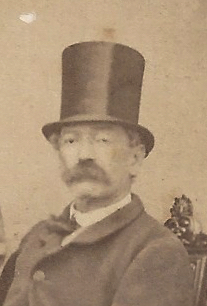
\includegraphics[height=7cm]{Fedele} }}%
    \subfloat[Natale Mingazzi]{{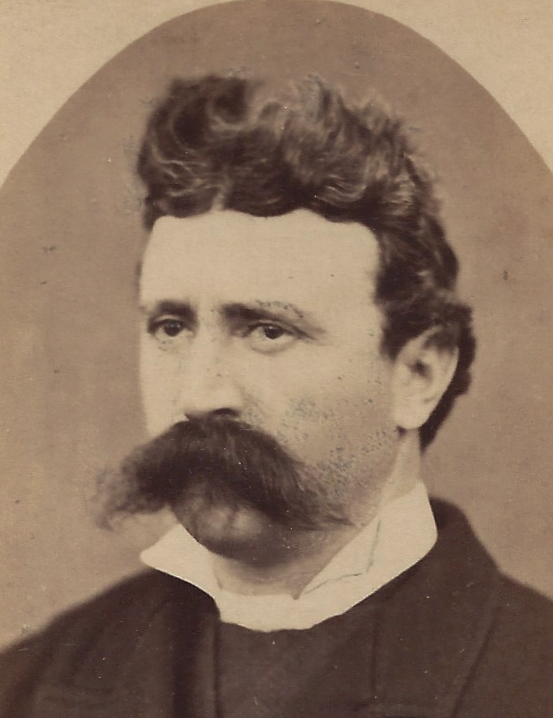
\includegraphics[height=7cm]{Natale} }}%
    \caption[Fedele e Natale Mingazzi]{}
	\vspace{-0.9cm}
\end{figure}

Ho immaginato quindi che Stefano, abbia riportato fedelmente le storie tramandate dal padre e dal nonno, per poi integrare l'opera con le sue esperienze personali.
Inoltre le ultime, benché siano presenti nell'indice, non sono mai state scritte per ovvi motivi. Ho deciso quindi di trascrivere tutte le storielle e di commentarle attingendo informazioni dalle fonti citate nel capitolo \textit{\nameref{fonti} }a pagina \pageref{fonti}.\\

Benché siano storielle palesemente sciocche, presentano parecchi dettagli dell'Alfonsine prebellica e della vita di fine `800 e inizio `900 che sono curiose ed interessanti.



